\documentclass[handout,xcolor=pdftex,dvipsnames,table]{beamer}\usepackage[]{graphicx}\usepackage[]{color}
%% maxwidth is the original width if it is less than linewidth
%% otherwise use linewidth (to make sure the graphics do not exceed the margin)
\makeatletter
\def\maxwidth{ %
  \ifdim\Gin@nat@width>\linewidth
    \linewidth
  \else
    \Gin@nat@width
  \fi
}
\makeatother

\definecolor{fgcolor}{rgb}{0.345, 0.345, 0.345}
\newcommand{\hlnum}[1]{\textcolor[rgb]{0.686,0.059,0.569}{#1}}%
\newcommand{\hlstr}[1]{\textcolor[rgb]{0.192,0.494,0.8}{#1}}%
\newcommand{\hlcom}[1]{\textcolor[rgb]{0.678,0.584,0.686}{\textit{#1}}}%
\newcommand{\hlopt}[1]{\textcolor[rgb]{0,0,0}{#1}}%
\newcommand{\hlstd}[1]{\textcolor[rgb]{0.345,0.345,0.345}{#1}}%
\newcommand{\hlkwa}[1]{\textcolor[rgb]{0.161,0.373,0.58}{\textbf{#1}}}%
\newcommand{\hlkwb}[1]{\textcolor[rgb]{0.69,0.353,0.396}{#1}}%
\newcommand{\hlkwc}[1]{\textcolor[rgb]{0.333,0.667,0.333}{#1}}%
\newcommand{\hlkwd}[1]{\textcolor[rgb]{0.737,0.353,0.396}{\textbf{#1}}}%

\usepackage{framed}
\makeatletter
\newenvironment{kframe}{%
 \def\at@end@of@kframe{}%
 \ifinner\ifhmode%
  \def\at@end@of@kframe{\end{minipage}}%
  \begin{minipage}{\columnwidth}%
 \fi\fi%
 \def\FrameCommand##1{\hskip\@totalleftmargin \hskip-\fboxsep
 \colorbox{shadecolor}{##1}\hskip-\fboxsep
     % There is no \\@totalrightmargin, so:
     \hskip-\linewidth \hskip-\@totalleftmargin \hskip\columnwidth}%
 \MakeFramed {\advance\hsize-\width
   \@totalleftmargin\z@ \linewidth\hsize
   \@setminipage}}%
 {\par\unskip\endMakeFramed%
 \at@end@of@kframe}
\makeatother

\definecolor{shadecolor}{rgb}{.97, .97, .97}
\definecolor{messagecolor}{rgb}{0, 0, 0}
\definecolor{warningcolor}{rgb}{1, 0, 1}
\definecolor{errorcolor}{rgb}{1, 0, 0}
\newenvironment{knitrout}{}{} % an empty environment to be redefined in TeX

\usepackage{alltt} 

\usecolortheme[RGB={0,0,144}]{structure}
%\usetheme{AnnArbor}\usecolortheme{beaver}
\usetheme{CambridgeUS}\usecolortheme{dolphin}
\usepackage{graphicx}
\usepackage[space]{grffile}
\usepackage{verbatim,xmpmulti,color,multicol,multirow}
\setlength{\unitlength}{\textwidth}  % measure in textwidths
\usepackage[normalem]{ulem}
\usepackage{amssymb,amsmath,latexsym}
\usepackage{booktabs}
\usepackage{array}
\newcolumntype{L}{>{$}l<{$}}
\newcolumntype{C}{>{$}c<{$}}
\newcolumntype{R}{>{$}r<{$}}
\newcommand{\nm}[1]{\textnormal{#1}}


%\usepackage{beamerthemesplit}
\setbeamertemplate{navigation symbols}{}
\setbeamertemplate{caption}[numbered]
%\setbeamercolor{alerted text}{fg=red}
%\setbeamertemplate{block body theorem}{bg=orange}
\setkeys{Gin}{width=0.6\textwidth}


%\SweaveOpts{concordance=TRUE}







\title[RNASeq Analysis]{Analyze RNASeq Data from G8P2 RFI (Residual Feed Intake) Lines Using QuasiSeq Package}


% \author[Yet Nguyen, Dan Nettleton]{Yet Nguyen \and Dan Nettleton}
% \institute[ISU]{Iowa State University}

%
\IfFileExists{upquote.sty}{\usepackage{upquote}}{}

\begin{document}
\frame{\maketitle}
\frame {
\frametitle{Table of Contents}
\begin{itemize}
\setlength{\itemsep}{.2in}
\item[1.] Data Summary
\item[2.] Model Selection Stragegies
\begin{itemize}
\item Number of genes with pvalues less than 0.05
\item Distance between Grenander CDF Estimator to Uniform CDF using
\begin{itemize}
\item Anderson-Darling Statistics
\item Crames-Von-Miser statistics
\item Kolmogorow-Smirnov statistics 
\end{itemize}
\end{itemize}
\item[3.] Results
\end{itemize}
}


\section{Data Summary}
\begin{frame}[fragile]
\frametitle{RNASeq Data Summary}
\begin{itemize}
\setlength{\itemsep}{.25in}
\item RNASeq data set is a  25322 $\times$ 24 table of count data  corresponding to 25322 genes of 24  pigs from 2 Lines: high RFI Line and low RFI Line, and 2 Diets: high energy diet (Diet 1) and low energy diet (Diet 2).

\item  There are 6 pigs for each combination of Diet and Line.
 
\end{itemize}
 

\end{frame}




%%%%%%%%%%%%%%%%
\frame{
\frametitle{Metadata Summary}
\begin{itemize}
\setlength{\itemsep}{.25in}
\item The available metadata consists of infomation of  9 covariates for 24 samples of 24 pigs.

\begin{itemize}
\item Factors: Diet (2 levels), Line (2 levels), Lane (2 levels), dateRNA (3 levels), and dateGD (5 levels).
\item Quantitative covariates: RFI (RFI values) , RINb (RNA Integrity Number before globin depletion), RINa (RNA Integrity Number after globin depletion), Conc (RNA Concentration after globin depletion).
\end{itemize}

\end{itemize}
}
%%%%%%%%%%%%%%%%%%%%%%%%%%%%%%%%%%%%%%%%%%%5

\frame{
\frametitle{Number of Genes Used in Analysis}
\begin{itemize}

\setlength{\itemsep}{.25in}


\item Models with metadata covariates: The number of genes analyzed is 14781. Those are genes with average counts greater than 1 and for which there are at least four samples with non-zero counts. 
\end{itemize}
}


%%%%%%%%%%%%%%%%%%%%%%%%%%%%%%%%%%%%%%%%%%%%%%%%%%%%%
\section{Model Selection}
\begin{frame}
\frametitle{Model Selection Criteria}
Starting model includes all interested covariates. For each covariate, 
\begin{itemize}
\setlength{\itemsep}{.2in}
\item We conduct a Likelihood Ratio Test using QuasiSeq of the full model vs. the reduced model obtained from the full model by deleting the considerated covariate. We collect the set of pvalues of all genes from the tests. 

\item Obtain the number of genes with pvalues less than or equal 0.05. 
\item Obtain Grenander CDF estimator of the empirical CDF of the sample from those pvalues.
\item Obtain the Anderson-Darling statistics, Crames-Von-Miser statistics, and Kolmogorow-Smirnov statistics between the Grenander CDF and uniform CDF.
\end{itemize}
Exclude the covariate corresponding to the smallest value for most of the above criteria.
\end{frame}
\begin{frame}[fragile]
\frametitle{Backward Model Selection}
\begin{figure}[h!]
    \centering
    %\includegraphics[width=\textwidth,height=0.8\textheight,keepaspectratio]{/home/ntyet/research/RFI-newdata/analysis/rfi/Plot06_26_2014_1.pdf}
    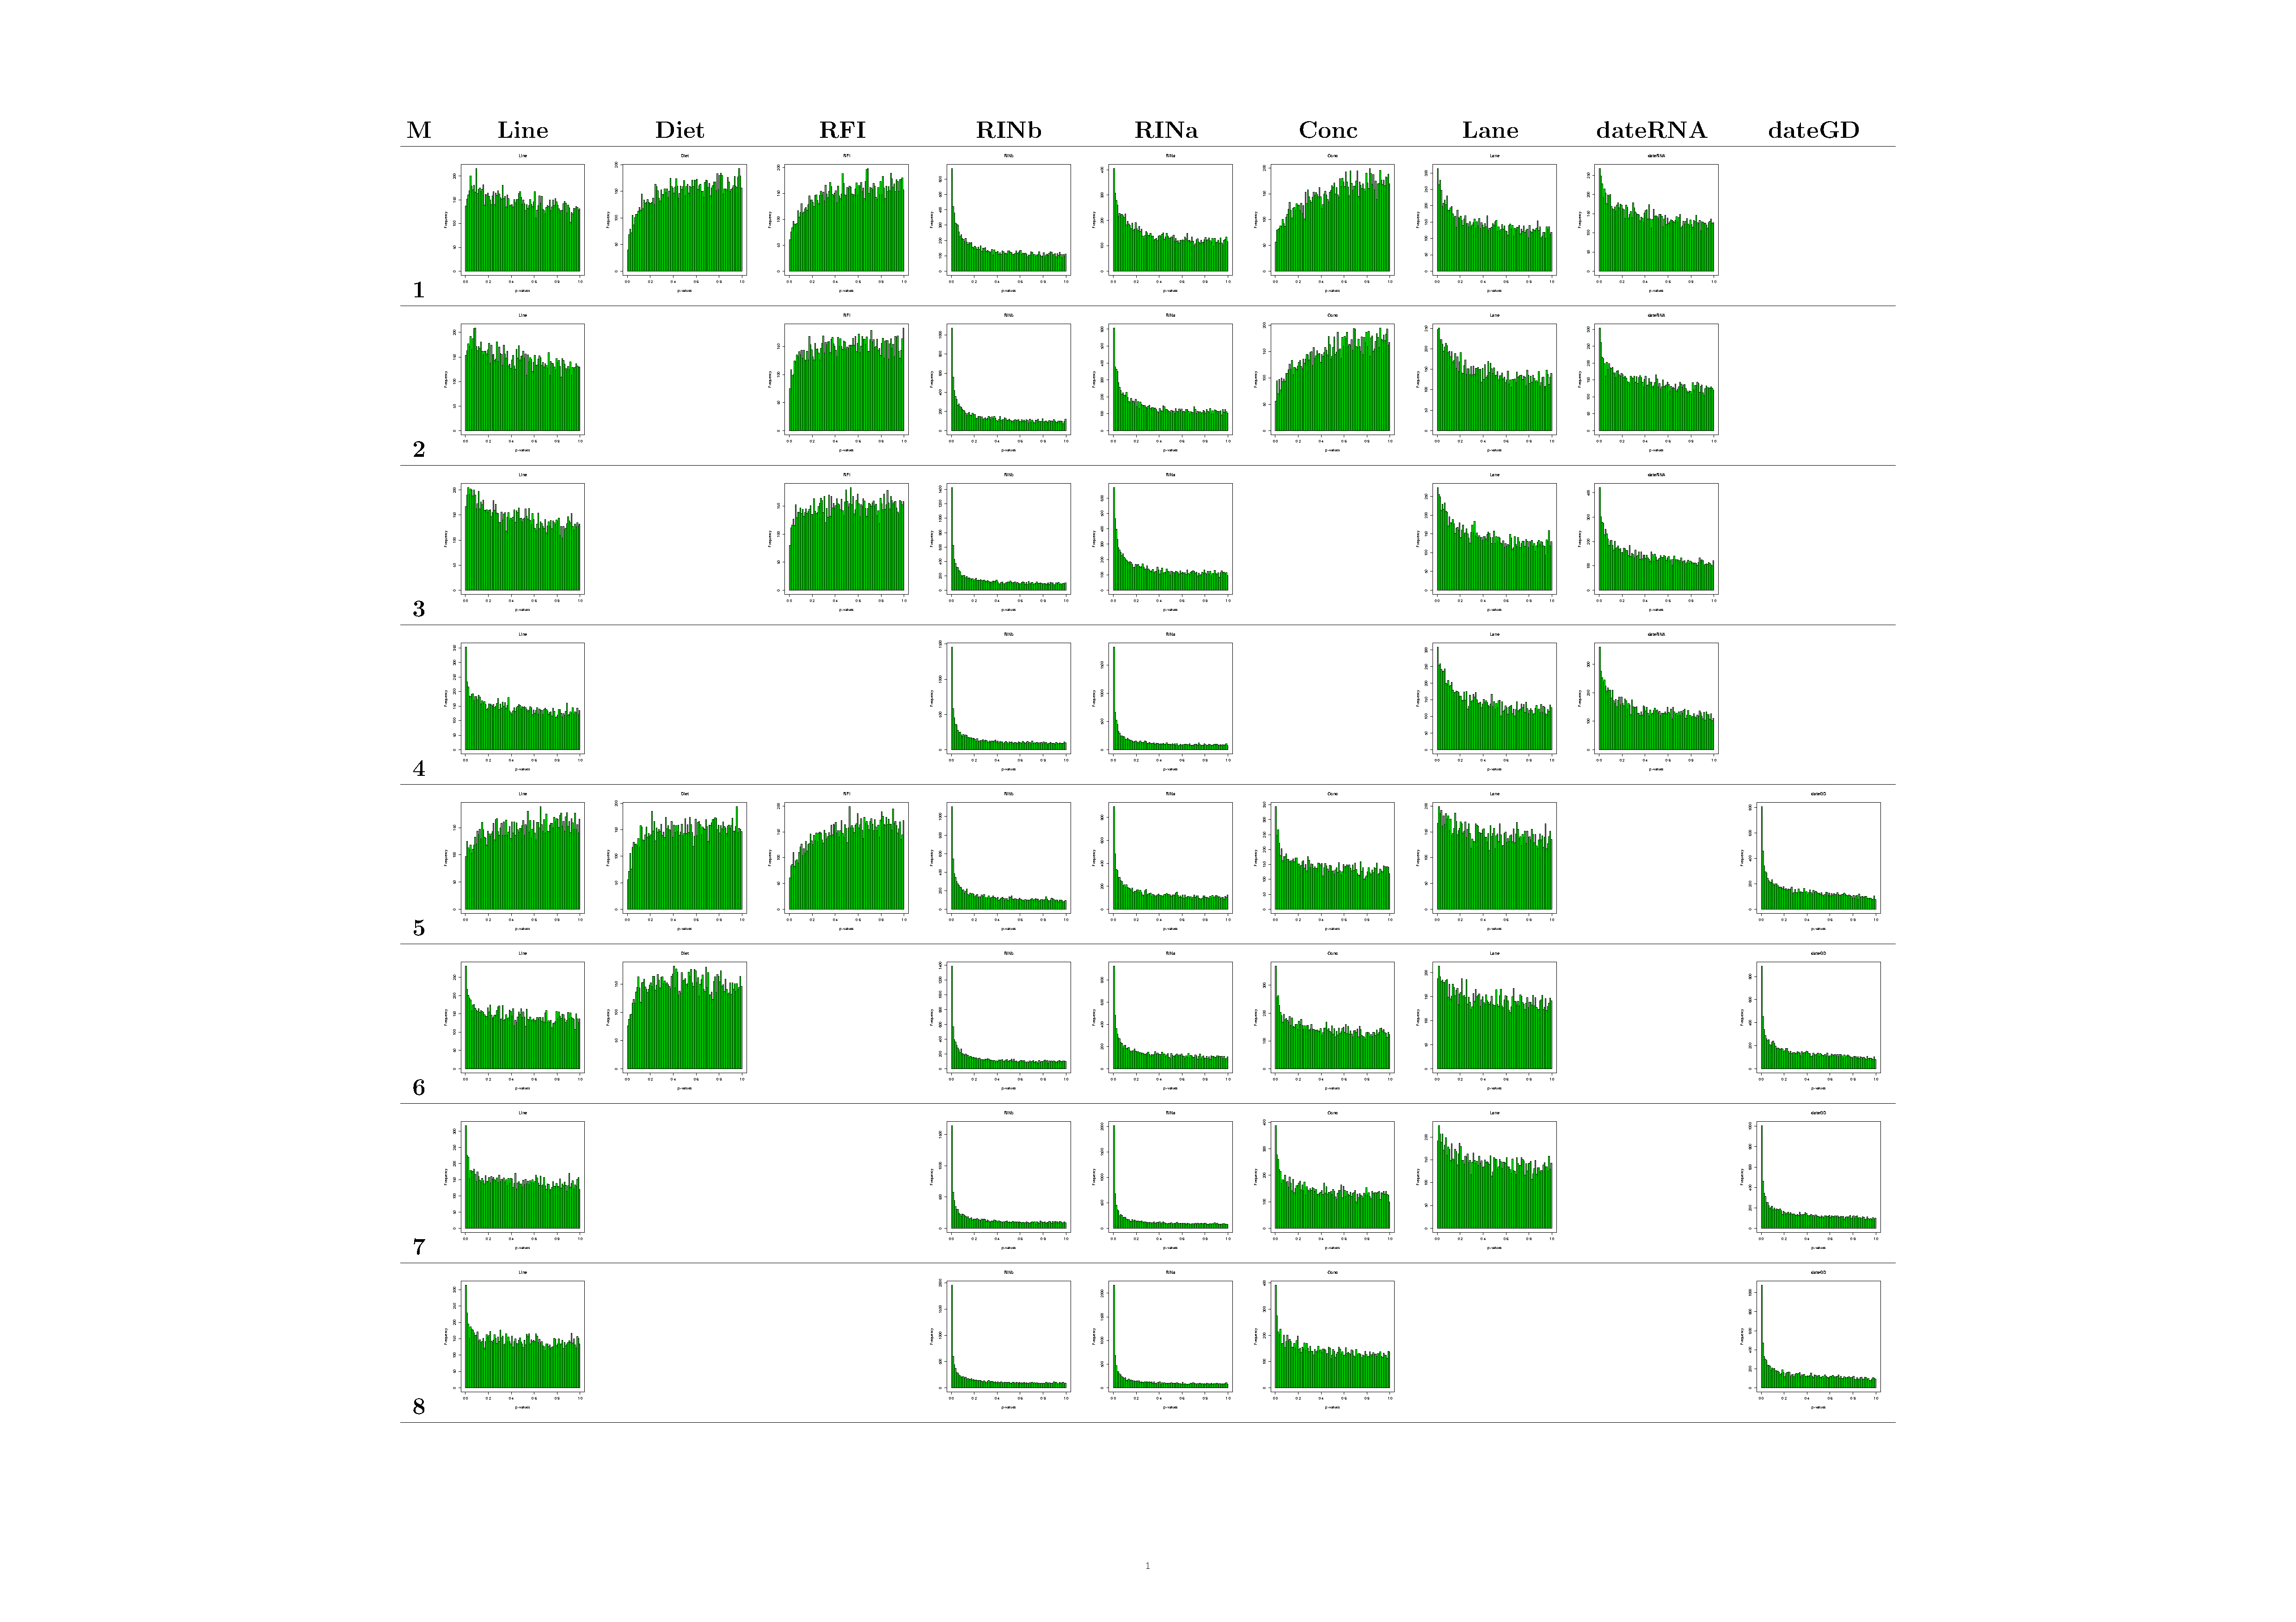
\includegraphics[width=\textwidth,height=1\textheight,keepaspectratio]{Plotmodel.pdf}
    \end{figure}
\end{frame}
\section{Results}
\begin{frame}[fragile]
\frametitle{Results of Model 4 and Model 8}
When FDR is controlled at 0.05, 0.10, 0.15, the number of DE Genes
between two RFI Lines (DEGs) and the number of DE Genes between
two RFI Lines with log(fold change) at least 1 (log(FC) ≥ 1) are
shown in the tables below









\begin{table}[htb]
\begin{minipage}{.45\textwidth}
\centering
% latex table generated in R 3.1.0 by xtable 1.7-3 package
% Fri Jul 11 14:21:42 2014
\begin{tabular}{rrr}
  \toprule
FDR & DEGs & $\mbox{log(FC)}\geq 1$ \\ 
  \midrule
0.05 &   0 &   0 \\ 
  0.10 &  10 &   2 \\ 
  0.15 &  23 &   5 \\ 
  0.20 &  60 &   8 \\ 
   \bottomrule
\end{tabular}


\captionof{Model 4: }{Estimated number of DE Genes between 2 Lines is 1965.}
\end{minipage}
\begin{minipage}{.45\textwidth}
\centering
% latex table generated in R 3.1.0 by xtable 1.7-3 package
% Fri Jul 11 14:21:42 2014
\begin{tabular}{rrr}
  \toprule
FDR & DEGs & $\mbox{log(FC)}\geq 1$ \\ 
  \midrule
0.05 &   3 &   1 \\ 
  0.10 &   6 &   1 \\ 
  0.15 &  28 &   3 \\ 
  0.20 &  45 &   4 \\ 
   \bottomrule
\end{tabular}


\captionof{Model 8: }{Estimated number of DE Genes between 2 Lines is 1172.}
\end{minipage}
\end{table}


\end{frame}
\begin{frame}[fragile]
\frametitle{Model 4 and Model 8 Pvalues of Line Effects }
\begin{knitrout}\footnotesize
\definecolor{shadecolor}{rgb}{0.969, 0.969, 0.969}\color{fgcolor}

{\centering \includegraphics[width=.6\linewidth]{figure/beamer-unnamed-chunk-1} 

}



\end{knitrout}


\end{frame}
\end{document}
